%%%%%%%% ICML 2023 EXAMPLE LATEX SUBMISSION FILE %%%%%%%%%%%%%%%%%

\documentclass{article}

% Recommended, but optional, packages for figures and better typesetting:
\usepackage{microtype}
\usepackage{graphicx}
\usepackage[export]{adjustbox}
\usepackage{tikz}
\usetikzlibrary{arrows.meta,positioning}
\usepackage{subfigure}
\usepackage{booktabs} % for professional tables

% hyperref makes hyperlinks in the resulting PDF.
% If your build breaks (sometimes temporarily if a hyperlink spans a page)
% please comment out the following usepackage line and replace
% \usepackage{icml2023} with \usepackage[nohyperref]{icml2023} above.
\usepackage{hyperref}


% Attempt to make hyperref and algorithmic work together better:
\newcommand{\theHalgorithm}{\arabic{algorithm}}

% Use the following line for the initial blind version submitted for review:
\usepackage[accepted]{styles/icml2023}

% If accepted, instead use the following line for the camera-ready submission:
% \usepackage[accepted]{icml2023}

% For theorems and such
\usepackage{amsmath}
\usepackage{amssymb}
\usepackage{mathtools}
\usepackage{amsthm}

% if you use cleveref..
\usepackage[capitalize,noabbrev]{cleveref}

%%%%%%%%%%%%%%%%%%%%%%%%%%%%%%%%
% THEOREMS
%%%%%%%%%%%%%%%%%%%%%%%%%%%%%%%%
\theoremstyle{plain}
\newtheorem{theorem}{Theorem}[section]
\newtheorem{proposition}[theorem]{Proposition}
\newtheorem{lemma}[theorem]{Lemma}
\newtheorem{corollary}[theorem]{Corollary}
\theoremstyle{definition}
\newtheorem{definition}[theorem]{Definition}
\newtheorem{assumption}[theorem]{Assumption}
\theoremstyle{remark}
\newtheorem{remark}[theorem]{Remark}

% Todonotes is useful during development; simply uncomment the next line
%    and comment out the line below the next line to turn off comments
%\usepackage[disable,textsize=tiny]{todonotes}
\usepackage[textsize=tiny]{todonotes}


% The \icmltitle you define below is probably too long as a header.
% Therefore, a short form for the running title is supplied here:
\icmltitlerunning{Generative Adversarial Networks on Flowers 102}

\begin{document}

\twocolumn[
\icmltitle{Training NeuralNector with \\
           Generative Adversarial Networks on Flowers 102}

% It is OKAY to include author information, even for blind
% submissions: the style file will automatically remove it for you
% unless you've provided the [accepted] option to the icml2023
% package.

% List of affiliations: The first argument should be a (short)
% identifier you will use later to specify author affiliations
% Academic affiliations should list Department, University, City, Region, Country
% Industry affiliations should list Company, City, Region, Country

% You can specify symbols, otherwise they are numbered in order.
% Ideally, you should not use this facility. Affiliations will be numbered
% in order of appearance and this is the preferred way.
\icmlsetsymbol{equal}{*}

\begin{icmlauthorlist}
\icmlauthor{Issac Roy}{ucsd}
\end{icmlauthorlist}

\icmlaffiliation{ucsd}{University of California, San Diego, La Jolla, USA}

\icmlcorrespondingauthor{Issac Roy}{iroy@ucsd.edu, ucsd}

% You may provide any keywords that you
% find helpful for describing your paper; these are used to populate
% the "keywords" metadata in the PDF but will not be shown in the document
\icmlkeywords{Generative Adversarial Networks, Flowers 102, MNIST, CIFAR-10}

\vskip 0.3in
]

% this must go after the closing bracket ] following \twocolumn[ ...

% This command actually creates the footnote in the first column
% listing the affiliations and the copyright notice.
% The command takes one argument, which is text to display at the start of the footnote.
% The \icmlEqualContribution command is standard text for equal contribution.
% Remove it (just {}) if you do not need this facility.

\printAffiliationsAndNotice{}  % leave blank if no need to mention equal contribution
% \printAffiliationsAndNotice{\icmlEqualContribution} % otherwise use the standard text.

\begin{figure}[t]
\vskip 0.1in
\begin{center}
\centerline{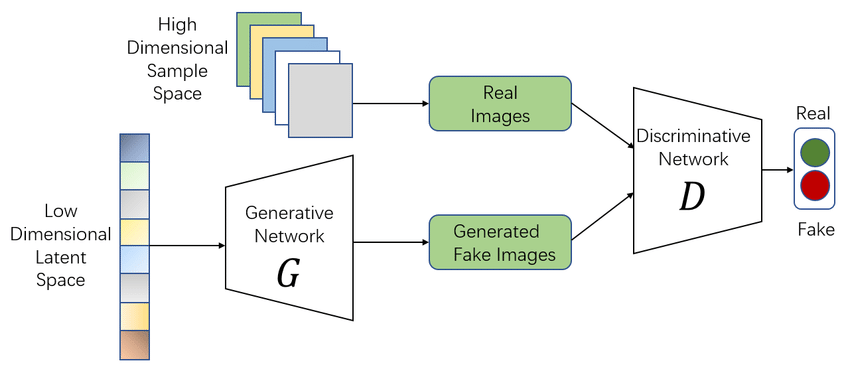
\includegraphics[width=\columnwidth]{images/GAN_architecture}}
\caption{High-level GAN setup: the generator maps latent noise to images; the discriminator scores real vs.\ fake.}
\label{fig:gan-arch}
\end{center}
\end{figure}

\begin{abstract}
This work trains DCGAN-style generative adversarial networks on MNIST and Oxford Flowers~102, progressing from a compact architecture for $28\times 28$ digits to a deeper convolutional generator and discriminator for $64\times 64$ RGB flower images. The resulting flower generator is deployed in \underline{\href{https://neuralnector.com}{NeuralNector}}, an interactive game in which human players act as the discriminator on grids of real versus synthetic images. Training is discussed in light of practical difficulties including discriminator dominance, vanishing gradients, and mode collapse, together with stabilizing modifications to the optimization procedure.
\end{abstract}

\section{Introduction}

Generative adversarial networks (GANs) \cite{GANs} are a framework for learning a model of a data distribution by pitting two neural networks against each other.
A \emph{generator} $G$ maps samples $z$ from a simple prior (e.g., Gaussian noise) to synthetic data $G(z)$ in the same space as real examples $x$.
A \emph{discriminator} $D$ is a classifier trained to distinguish real data from generated samples.
Training alternates between updating $D$ to assign high probability to real $x$ and low probability to $G(z)$, and updating $G$ to produce samples that fool $D$.
\cref{fig:gan-arch} sketches the adversarial setup and layer structure used in this work.

The original minimax objective \cite{GANs} is
\begin{equation}
\label{eq:gan-minimax}
\min_G \max_D \;
\mathbb{E}_{x \sim p_{\mathrm{data}}}[\log D(x)]
+ \mathbb{E}_{z \sim p_z}[\log (1 - D(G(z)))]\,,
\end{equation}
where $D(x) \in (0,1)$ is interpreted as the probability that $x$ is real.
In practice, $G$ is often trained with a \emph{non-saturating} loss that maximizes $\mathbb{E}_z[\log D(G(z))]$ instead of minimizing $\mathbb{E}_z[\log(1-D(G(z)))]$, which can mitigate vanishing gradients when $D$ rejects fakes with high confidence \cite{GANs}.
Our implementation follows the standard recipe of optimizing $D$ and $G$ with alternating stochastic gradient steps on losses equivalent to binary cross-entropy between $D$'s output and labels for real vs.\ fake batches (with additional stabilizers described in \cref{sec:methods}). However, we found that the discriminator can become too accurate too quickly, which yields vanishing gradients for $G$ and stalled learning \cite{TrainingGANs,ImprovedGANs}. Our solution is to skip the discriminator update if the discriminator's loss dips below a certain threshold, allowing $G$ to catch up.

GAN training is notoriously fragile.
As mentioned above, the discriminator can become too accurate too quickly, which yields vanishing gradients for $G$ and stalled learning.
\emph{Mode collapse} occurs when $G$ maps many latent vectors to a small set of outputs, limiting diversity \cite{TrainingGANs,ImprovedGANs}. \cref{fig:mode-collapse} shows an example of mode collapse on the Flowers 102 dataset where the generator only produces white images.
Other pathologies include oscillations and sensitivity to hyperparameters \cite{TrainingGANs}.
These issues motivated a large body of follow-on work (e.g., improved optimization and evaluation \cite{ImprovedGANs,WassersteinGAN}); in this project we address practical instability with architectural scaling and training heuristics rather than attempting to formulate a new objective.

We began with the MNIST dataset and a compact convolutional architecture in \texttt{GAN\_MNIST.ipynb}: a shallow discriminator with convolutions, pooling, and fully connected layers, and a generator built from a linear projection to a small spatial grid followed by transposed convolutions to produce $28\times 28$ grayscale digits.
We then moved to the Oxford Flowers~102 dataset \cite{Nilsback08}, which is substantially harder: natural color images at higher resolution require a deeper DCGAN-style design with more layers and $64\times 64$ RGB outputs, developed in \texttt{GAN\_pytorch.ipynb}.
On Flowers we observed vanishing gradients, mode collapse, and a discriminator that reached near-optimality too early, suppressing learning in $G$.
We mitigated these effects with practices such as label smoothing, asymmetric learning rates for $G$ and $D$, and selective updates that skip or repeat discriminator steps when its loss indicates it is overpowering the generator; details appear in \cref{sec:methods}.
The resulting generator powers \underline{\href{https://neuralnector.com}{NeuralNector}}, an interactive game in which human players act as discriminators on grids of real vs.\ GAN-generated flowers.

\begin{figure}[t]
\vskip 0.1in
\begin{center}
\centerline{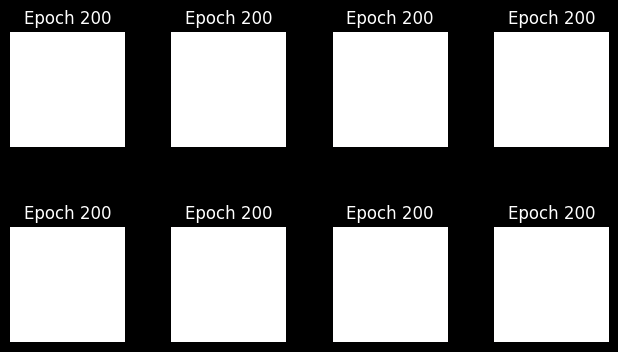
\includegraphics[width=\columnwidth]{images/flower_collapse}}
\caption{Mode collapse in the generator on the Flowers 102 dataset causes only white images to be generated.}
\label{fig:mode-collapse}
\end{center}
\vskip -0.4in
\end{figure}

\begin{figure}[t]
\vskip 0.1in
\begin{center}
\centerline{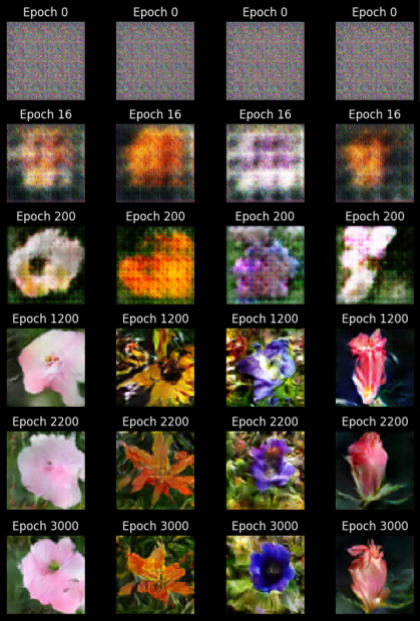
\includegraphics[width=\columnwidth]{images/epochs}}
\caption{Samples from the generator at selected training epochs (flowers).}
\label{fig:training-epochs}
\end{center}
\vskip -0.4in
\end{figure}

\section{Methods}
\label{sec:methods}

All models are implemented in PyTorch with the PyTorch Lightning training framework, using manual optimization so the generator and discriminator can be updated on different schedules with distinct learning rates.

\subsection{Datasets and splits}

\paragraph{MNIST.}
Grayscale digits are resized to $28\times 28$. Inputs use the standard per-channel normalization to match the mean and variance. The training partition is split into approximately $55{,}000$ training and $5{,}000$ validation examples; the held-out test set is reserved for qualitative checks. This setting is used to validate the training loop and a lightweight convolutional architecture before scaling to natural images.

\paragraph{Oxford Flowers~102 \cite{Nilsback08}.}
Images are resized and cropped to $64\times 64$ RGB. Pixel values are mapped to $[-1,1]$ via normalization with mean and standard deviation $0.5$ per channel, which matches the \texttt{tanh} output range of the generator.
The dataset provides only about $1{,}000$ images in each of the official training and validation splits; to increase per-epoch diversity and exposure to the class distribution, the training and validation splits are concatenated for optimization. The official test split isn't used during training and is kept for evaluation in \cref{sec:experiments}.
When training, optional data augmentation (random crops, flips, jitter, etc.) further increases variability for the flower domain.

\subsection{Architectures: MNIST vs.\ Flowers}
% Each dataset: Generator (left) and Discriminator (right) side by side.
\begin{figure*}[t]
\vskip -0.05in
\centering
\footnotesize
\tikzset{
  ganbox/.style={rectangle, draw=black!70, line width=0.45pt, rounded corners=2pt,
    inner sep=1.4pt, align=center, font={\fontsize{6.5}{7.6}\selectfont}, text width=1.92cm, minimum height=0.44cm},
  ganarr/.style={-{Stealth[length=1.25mm]}, semithick, black!55, shorten >=0.4pt, shorten <=0.4pt},
}
\begin{adjustbox}{max width=\textwidth, max height=0.88\textheight, center}
% ---------- MNIST ----------
\begin{minipage}[t]{0.48\textwidth}
\centering
{\small MNIST} \quad {\footnotesize\itshape $28{\times}28$, 1 ch.}\\[0.35em]
\noindent
\begin{minipage}[t]{0.49\linewidth}\centering
\textit{Generator}\\[0.12em]
\begin{tikzpicture}[node distance=1.45mm, >=Stealth]
  \node[ganbox] (mg1) {$\mathbf{z}$ batch$\times 100$};
  \node[ganbox, below=of mg1] (mg2) {Linear $\rightarrow$ reshape\\$64\times 7\times 7$, ReLU};
  \node[ganbox, below=of mg2] (mg3) {ConvT $64\!\to\!32$, $k{=}4$, $s{=}2$\\$7^2 \!\to\! 14^2$, ReLU};
  \node[ganbox, below=of mg3] (mg4) {ConvT $32\!\to\!16$, $k{=}4$, $s{=}2$\\$14^2 \!\to\! 28^2$, ReLU};
  \node[ganbox, below=of mg4] (mg5) {Conv $16\!\to\!1$, $k{=}7$\\\texttt{tanh} $\rightarrow 28^2$};
  \foreach \a/\b in {mg1/mg2,mg2/mg3,mg3/mg4,mg4/mg5} \draw[ganarr] (\a) -- (\b);
\end{tikzpicture}
\end{minipage}%
\hfill
\begin{minipage}[t]{0.49\linewidth}\centering
\textit{Discriminator}\\[0.12em]
\begin{tikzpicture}[node distance=1.45mm, >=Stealth]
  \node[ganbox] (md1) {$\mathbf{x}$ $1\times28\times28$};
  \node[ganbox, below=of md1] (md2) {Conv $1\!\to\!10$, $k{=}5$\\ReLU + max-pool\\$\rightarrow 10{\times}12^2$};
  \node[ganbox, below=of md2] (md3) {Conv $10\!\to\!20$, $k{=}5$\\Dropout2d + pool + ReLU\\$\rightarrow 20{\times}4^2$};
  \node[ganbox, below=of md3] (md4) {FC $320\!\to\!50$\\ReLU + dropout};
  \node[ganbox, below=of md4] (md5) {FC $50\!\to\!1$ + sigmoid};
  \foreach \a/\b in {md1/md2,md2/md3,md3/md4,md4/md5} \draw[ganarr] (\a) -- (\b);
\end{tikzpicture}
\end{minipage}
\end{minipage}%
\hfill
% ---------- Flowers ----------
\begin{minipage}[t]{0.48\textwidth}
\centering
{\small Flowers 102} \quad {\footnotesize\itshape $64{\times}64$, 3 ch.}\\[0.35em]
\noindent
\begin{minipage}[t]{0.49\linewidth}\centering
\textit{Generator}\\[0.12em]
\begin{tikzpicture}[node distance=1.35mm, >=Stealth]
  \node[ganbox] (fg1) {$\mathbf{z}$ batch$\times 100$};
  \node[ganbox, below=of fg1] (fg2) {Linear $\rightarrow$ reshape\\$512\times 4\times 4$, ReLU};
  \node[ganbox, below=of fg2] (fg3) {ConvT $512\!\to\!256$, $k{=}4$, $s{=}2$\\+ BN + ReLU $\rightarrow 8^2$};
  \node[ganbox, below=of fg3] (fg4) {ConvT $256\!\to\!128$, $s{=}2$\\+ BN + ReLU $\rightarrow 16^2$};
  \node[ganbox, below=of fg4] (fg5) {ConvT $128\!\to\!64$, $s{=}2$\\+ BN + ReLU $\rightarrow 32^2$};
  \node[ganbox, below=of fg5] (fg6) {ConvT $64\!\to\!32$, $s{=}2$\\+ BN + ReLU $\rightarrow 64^2$};
  \node[ganbox, below=of fg6] (fg7) {Conv $32\!\to\!3$, $k{=}3$, pad 1\\\texttt{tanh}};
  \foreach \a/\b in {fg1/fg2,fg2/fg3,fg3/fg4,fg4/fg5,fg5/fg6,fg6/fg7} \draw[ganarr] (\a) -- (\b);
\end{tikzpicture}
\end{minipage}%
\hfill
\begin{minipage}[t]{0.49\linewidth}\centering
\textit{Discriminator}\\[0.12em]
\begin{tikzpicture}[node distance=1.45mm, >=Stealth]
  \node[ganbox] (fd1) {$\mathbf{x}$ $3\times64\times64$};
  \node[ganbox, below=of fd1] (fd2) {Conv $3\!\to\!64$, $k{=}4$, $s{=}2$\\LeakyReLU (no BN)\\$\rightarrow 32^2$};
  \node[ganbox, below=of fd2] (fd3) {Conv $64\!\to\!128$, $s{=}2$\\+ BN + LeakyReLU $\rightarrow 16^2$};
  \node[ganbox, below=of fd3] (fd4) {Conv $128\!\to\!256$, $s{=}2$\\+ BN + LeakyReLU $\rightarrow 8^2$};
  \node[ganbox, below=of fd4] (fd5) {Conv $256\!\to\!512$, $s{=}2$\\+ BN + LeakyReLU $\rightarrow 4^2$};
  \node[ganbox, below=of fd5] (fd6) {Flatten + FC\\$4{\cdot}4{\cdot}512 \!\to\! 1$ + sigmoid};
  \foreach \a/\b in {fd1/fd2,fd2/fd3,fd3/fd4,fd4/fd5,fd5/fd6} \draw[ganarr] (\a) -- (\b);
\end{tikzpicture}
\end{minipage}
\end{minipage}
\end{adjustbox}
\vskip 0.08in
\caption{Neural architectures (\texttt{models.py}). \emph{Left:} MNIST---$G$ and $D$ side by side; shallow $D$ (pooling, dropout, no BN); $G$ without BN. \emph{Right:} Flowers---DCGAN-style $D$ (BN except first conv, LeakyReLU) and $G$ (transposed convs + BN + ReLU, \texttt{tanh}).}
\label{fig:gan-arch}
\vskip -0.1in
\end{figure*}


The same conceptual GAN objective (\cref{eq:gan-minimax}) is used throughout; the capacity and inductive bias of the networks are scaled with dataset difficulty.
\cref{fig:gan-arch} summarizes the layer stacks for both regimes, with $G$ and $D$ drawn side by side within each panel.

\paragraph{MNIST ($28\times 28$, 1 channel).}
The discriminator is a small CNN: two convolutional layers with $5\times 5$ kernels, max pooling, dropout on the second conv block, and two fully connected layers ending in a single logit passed through a sigmoid. This shallow design is sufficient for aligned digits and trains quickly while limiting overfitting on a simple domain.
The generator maps Gaussian noise of dimension $z\in\mathbb{R}^{100}$ through a linear layer to a $7\times 7\times 64$ tensor, applies two transposed convolutions to reach spatial size $28\times 28$, and a final convolution with \texttt{tanh}. Batch normalization is omitted in this path to keep the starter model minimal and to avoid small-batch noise on early experiments; ReLU activations are used in the generator, and ReLU with pooling in the discriminator.

\paragraph{Flowers ($64\times 64$, 3 channels).}
Natural color flowers exhibit richer texture and spatial structure, so both networks follow a DCGAN-style deep convolutional layout with strided convolutions in $D$ and transposed convolutions in $G$.
The discriminator stacks four strided $4\times 4$ convolutions with channel widths $64\!\to\!128\!\to\!256\!\to\!512$, batch normalization on all but the first layer (a common practice so the input statistics are not whitewashed), LeakyReLU ($0.2$) activations, and a linear layer to one output with sigmoid. BN and LeakyReLU help stabilize gradients when $D$ must discriminate fine-grained natural detail; the first conv remains unnormalized so the network can learn low-level edge statistics directly from pixels.
The generator projects $z\in\mathbb{R}^{100}$ to $4\times 4\times 512$, then upsamples through four transposed convolution stages ($512\!\to\!256\!\to\!128\!\to\!64\!\to\!32$ feature maps) each followed by batch normalization and ReLU, and a final $3\times 3$ convolution to three channels with \texttt{tanh}. BN in $G$ reduces internal covariate shift across upsampling stages and tends to improve training stability when many layers are stacked.

Convolutional, transposed-convolutional, and linear weights are initialized from $\mathcal{N}(0, 0.02^2)$ with zero bias initialization, following common GAN practice.

\subsection{Loss and alternating updates}

The discriminator is trained to minimize binary cross-entropy between its sigmoid output and soft targets for real vs.\ fake batches. Label smoothing with parameter $0.1$ replaces hard labels $1$ and $0$ for real and fake with $0.9$ and $0.1$, which discourages $D$ from becoming overconfident and mitigates vanishing gradients through the generator when fakes are trivially rejected \cite{ImprovedGANs}.
The generator is trained to fool $D$, using BCE against targets of ``real'' ($1$) for generated samples (non-saturating form, consistent with \cref{eq:gan-minimax} and the discussion in the introduction).

\subsection{Optimization and adaptive balancing}

Both networks use Adam with betas $(0.5, 0.999)$. The base learning rate is $2\times 10^{-4}$ for the hyperparameter \texttt{lr}, but asymmetric effective rates are applied: the generator uses \texttt{lr}$_{\!G}=2\times$\texttt{lr} ($4\times 10^{-4}$) and the discriminator \texttt{lr}$_{\!D}=\frac{1}{2}\times$\texttt{lr} ($1\times 10^{-4}$). The intent is to slow $D$ and accelerate $G$ so the discriminator does not reach optimality too quickly---a regime in which $G$ receives little useful gradient and training stalls.

Additional adaptive scheduling is implemented in the training step: if the averaged discriminator loss $d_{\mathrm{loss}}$ falls below $0.6$, the discriminator update for that step is skipped ($D$ is already winning too easily; updating it further would harm $G$). If $d_{\mathrm{loss}}$ falls below $0.4$, the generator is updated twice in one step (second draw of $z$) so $G$ can recover when $D$ is very strong.
Together with label smoothing and asymmetric learning rates, this implements a simple heuristic schedule that pauses or emphasizes updates based on the relative strength of $D$ and $G$, without changing the underlying minimax game.

Typical batch sizes are $128$ for early MNIST experiments in \texttt{GAN\_MNIST.ipynb} and $64$ for Flowers in \texttt{GAN\_pytorch.ipynb}, subject to GPU memory.

\subsection{Selecting fakes for NeuralNector}

After training, synthetic flowers for the web game are produced by sampling the generator and ranking candidates by the discriminator's output, interpreted as the model's estimated probability that an image is real. A large pool of candidates is generated (and optionally merged with previously generated images), all are scored under a fixed checkpoint, and the top $500$ by discriminator score are written to the game's fake image archive. This heuristic filters out egregious failures and mode-collapsed samples that $D$ confidently rejects, improving the quality of the human-facing ``fake'' set at the cost of biasing the pool toward samples the current $D$ finds plausible. The same trained \texttt{gan\_flowers\_final.ckpt} checkpoint is loaded in production for inference.

\begin{table}[t]
\caption{Default hyperparameters for Flowers~102 training (unless varied in \cref{sec:experiments}).}
\label{tab:hparams}
\vskip 0.1in
\begin{center}
\begin{small}
\begin{sc}
\begin{tabular}{lc}
\toprule
Setting & Value \\
\midrule
Latent dimension $|\mathbf{z}|$ & $100$ \\
Base \texttt{lr} & $2\times 10^{-4}$ \\
$\mathrm{lr}_G$ / $\mathrm{lr}_D$ & $2\times$ / $0.5\times$ base \\
Label smoothing & $0.1$ \\
Adam $(\beta_1,\beta_2)$ & $(0.5,\,0.999)$ \\
Skip $D$ step if $d_{\mathrm{loss}}<$ & $0.6$ \\
Extra $G$ step if $d_{\mathrm{loss}}<$ & $0.4$ \\
Flowers batch size & $64$ \\
Output activation & \texttt{tanh} on $G$, sigmoid on $D$ \\
\bottomrule
\end{tabular}
\end{sc}
\end{small}
\end{center}
\vskip -0.1in
\end{table}

\section{Experiments}
\label{sec:experiments}

We report a \emph{comparative} study using the same PyTorch Lightning training loop as in \cref{sec:methods}, with budgets chosen to keep total compute modest (about eleven minutes of GPU time on an NVIDIA A100 in our Colab run, summing eight configurations). These runs are \emph{not} intended to match the long Flowers training used for deployment (thousands of epochs in \texttt{GAN\_pytorch.ipynb}); instead they isolate how individual stabilizers affect optimization trajectories over a fixed short horizon. Unless noted, hyperparameters match \cref{tab:hparams}. Recorded quantities are the generator and discriminator losses logged at the end of each epoch (BCE-style objectives as implemented in the notebooks).

\subsection{MNIST training ablations}

On MNIST we train for $12$ epochs at batch size $128$ with the $28\times 28$ architecture from \cref{sec:methods}. \cref{tab:mnist-ablations} summarizes final losses and means over the last three epochs. Several ablations leave both losses in a similar band (roughly $L_G\approx 0.59$--$0.70$, $L_D\approx 0.58$--$0.59$): removing label smoothing (\texttt{M2}), using symmetric learning rates for $G$ and $D$ (\texttt{M3}), reducing the latent dimension to $50$ (\texttt{M5}), and raising Adam's $\beta_1$ to $0.9$ (\texttt{M6}). These differences are modest on this budget and should be interpreted cautiously---GAN losses need not correlate monotonically with sample quality.

The clearest signal is \texttt{M4\_always\_train\_D}, which disables the adaptive rule that skips discriminator updates when $d_{\mathrm{loss}}<0.6$ (implemented as a skip threshold of $-1$). Here the discriminator loss falls to about $0.34$ while the generator loss climbs to about $2.26$, with a monotonic upward trend in $L_G$ after the first epoch. This pattern is consistent with discriminator dominance: $D$ becomes too confident too quickly, which weakens the learning signal for $G$ under the non-saturating objective. The default schedule (\texttt{M1\_baseline}), which can pause $D$, avoids this failure mode on the same epoch budget. Together, these results support the narrative in the introduction: the heuristic balancing of $G$ and $D$ updates is not merely cosmetic; when removed, optimization behavior changes sharply even on a simple dataset.

Qualitatively, we inspected $8\times 8$ sample grids exported for each run (files \texttt{M1\_baseline.png}--\texttt{M6\_beta1\_0.9.png} under \texttt{experiment\_outputs/experiment\_grids/} in the accompanying notebook). The grids should be compared with the usual caveat that short-run MNIST GANs may already produce recognizable digits across settings; the quantitative table is most useful for relative optimization behavior, especially the \texttt{M4} contrast.

\begin{table}[t]
\caption{MNIST ablations ($12$ epochs, batch $128$). $L_G,L_D$: losses at the final epoch; $\bar{L}^{(3)}$: mean over the last three epochs. Wall time is per run on one GPU.}
\label{tab:mnist-ablations}
\vskip 0.1in
\begin{center}
\begin{small}
\begin{sc}
\begin{tabular}{lccccr}
\toprule
Run & $L_G$ & $L_D$ & $\bar{L}_G^{(3)}$ & $\bar{L}_D^{(3)}$ & s \\
\midrule
\texttt{baseline} & $0.697$ & $0.581$ & $0.689$ & $0.584$ & $93$ \\
\texttt{no\_label\_smooth} & $0.612$ & $0.578$ & $0.608$ & $0.580$ & $89$ \\
\texttt{symmetric\_lr} & $0.594$ & $0.585$ & $0.592$ & $0.586$ & $89$ \\
\texttt{always\_train\_D} & $2.258$ & $0.342$ & $2.239$ & $0.343$ & $113$ \\
\texttt{latent\_50} & $0.683$ & $0.585$ & $0.684$ & $0.585$ & $88$ \\
\texttt{beta1\_0.9} & $0.681$ & $0.585$ & $0.682$ & $0.585$ & $89$ \\
\bottomrule
\end{tabular}
\end{sc}
\end{small}
\end{center}
\vskip -0.1in
\end{table}

\subsection{Flowers: data augmentation}

On Flowers~102 we compare $10$ epochs at batch size $64$ with the $64\times 64$ DCGAN-style architecture, holding optimization hyperparameters fixed. \cref{tab:flowers-aug} contrasts the default recipe with augmentation enabled (\texttt{F1\_flowers\_baseline}) against the same setup with augmentation disabled (\texttt{F2\_flowers\_no\_aug}). On this short horizon, augmentation yields a lower final generator loss ($1.17$ vs.\ $1.43$) and a substantially lower mean generator loss over the last three epochs ($1.16$ vs.\ $2.60$), while discriminator losses remain in a similar range ($\approx 0.65$--$0.67$ at the end). The loss trace for \texttt{F2} is also more volatile (several mid-training spikes in $L_G$), which is consistent with reduced diversity of training views when only deterministic resizing/cropping is used.

As with MNIST, these numbers are proxies for optimization dynamics rather than a full perceptual evaluation; the main Flowers model in NeuralNector is trained far longer. Augmentation is retained in the default pipeline as a practical stabilizer for the natural-image regime.

\begin{table}[t]
\caption{Flowers~102 comparison ($10$ epochs, batch $64$). Aug.: random augmentation on vs.\ off. Notation as in \cref{tab:mnist-ablations}.}
\label{tab:flowers-aug}
\vskip 0.1in
\begin{center}
\begin{small}
\begin{sc}
\begin{tabular}{lccccc}
\toprule
Run & Aug. & $L_G$ & $L_D$ & $\bar{L}_G^{(3)}$ & $\bar{L}_D^{(3)}$ \\
\midrule
\texttt{baseline} & yes & $1.168$ & $0.652$ & $1.160$ & $0.664$ \\
\texttt{no\_aug} & no & $1.428$ & $0.667$ & $2.600$ & $0.740$ \\
\bottomrule
\end{tabular}
\end{sc}
\end{small}
\end{center}
\vskip -0.1in
\end{table}

\subsection{Limitations}

The study uses a single seed, does not report Inception score or FID, and relies on loss curves and informal grid inspection. Extending the same protocol with multiple seeds, longer budgets, and standard generative metrics would strengthen claims about sample quality; the present results are best read as evidence about \emph{optimization stability} and the role of specific heuristics under controlled ablations.

\section{Conclusion}
\label{sec:conclusion}

We implemented DCGAN-style adversarial training for MNIST and Oxford Flowers~102, scaling architecture and data pipeline with dataset difficulty, and documented practical failure modes (discriminator dominance, mode collapse) familiar from the GAN literature. Short-budget ablations corroborate that adaptive balancing of $G$ and $D$ updates matters even on MNIST (\cref{tab:mnist-ablations}), and that data augmentation tends to smooth Flowers optimization on a matched epoch budget (\cref{tab:flowers-aug}). The trained flower generator is deployed in NeuralNector, where human players discriminate real from synthetic images selected in part by discriminator scores.

Future work could add systematic evaluation (e.g., FID), sweep learning rates and thresholds more densely, and explore alternative objectives or regularizers while preserving the game's latency and data-pipeline constraints.


% In the unusual situation where you want a paper to appear in the
% references without citing it in the main text, use \nocite

\nocite{ConditionalGANs}
\nocite{VQGAN}
\nocite{UnderstandingGANs}
\nocite{MathBehindGANs}
\nocite{GANs}
\nocite{TrainingGANs}
\nocite{ImprovedGANs}
\nocite{WassersteinGAN}
\nocite{NDRL}
\nocite{NonLocalNets}

\bibliographystyle{icml2023}
\bibliography{main.bib}

\end{document}


% This document was modified from the file originally made available by
% Pat Langley and Andrea Danyluk for ICML-2K. This version was created
% by Iain Murray in 2018, and modified by Alexandre Bouchard in
% 2019 and 2021 and by Csaba Szepesvari, Gang Niu and Sivan Sabato in 2022.
% Modified again in 2023 by Sivan Sabato and Jonathan Scarlett.
% Previous contributors include Dan Roy, Lise Getoor and Tobias
% Scheffer, which was slightly modified from the 2010 version by
% Thorsten Joachims & Johannes Fuernkranz, slightly modified from the
% 2009 version by Kiri Wagstaff and Sam Roweis's 2008 version, which is
% slightly modified from Prasad Tadepalli's 2007 version which is a
% lightly changed version of the previous year's version by Andrew
% Moore, which was in turn edited from those of Kristian Kersting and
% Codrina Lauth. Alex Smola contributed to the algorithmic style files.
